\documentclass{beamer}

% To have the citation lists ordered by number.
\usepackage[nocompress]{cite}
\usepackage[utf8]{inputenc}
\usepackage{graphicx}
\usepackage[tight,TABTOPCAP]{subfigure}
\usepackage{amsmath}
\usepackage{amssymb}
\usepackage{amsfonts}
\usepackage{url}
\usepackage{proof}

\usepackage{hyperref}

\usepackage{tikz}
\usetikzlibrary{shapes.symbols}
\usetikzlibrary{shapes}
\usepackage{color}

\usepackage{color}
\usepackage{listings}
\lstset{ %
language=C,                % choose the language of the code
basicstyle=\footnotesize,       % the size of the fonts that are used for the code
numbers=left,                   % where to put the line-numbers
numberstyle=\footnotesize,      % the size of the fonts that are used for the line-numbers
stepnumber=1,                   % the step between two line-numbers. If it is 1 each line will be numbered
numbersep=5pt,                  % how far the line-numbers are from the code
backgroundcolor=\color{white},  % choose the background color. You must add \usepackage{color}
showspaces=false,               % show spaces adding particular underscores
showstringspaces=false,         % underline spaces within strings
showtabs=false,                 % show tabs within strings adding particular underscores
frame=single,   		% adds a frame around the code
tabsize=2,  		% sets default tabsize to 2 spaces
captionpos=b   		% sets the caption-position to bottom
}



%%%%%%%%%% Tool Names %%%%%%%%%%%%
\newcommand{\csisat}{{\sc CSIsat}}
\newcommand{\blast}{{\sc Blast}}
\newcommand{\armc}{{\sc ARMC}}
\newcommand{\mathsat}{{\sc MathSAT}}
\newcommand{\picosat}{{\sc PicoSAT}}
\newcommand{\clpprover}{{\sc CLPprover}}
\newcommand{\foci}{{\sc Foci}}
\newcommand{\sicstus}{{\sc SICStus Prolog}}

%%%%%%%%%% NOTATIONS %%%%%%%%%%%%
\newcommand{\true}{{\it true}}
\newcommand{\false}{{\it false}}
\newcommand{\sat}{{\sc sat}}
\newcommand{\laeuf}{{\sc LA+EUF}}

\renewcommand{\implies}{\Rightarrow}


\mode<presentation>
{
  \usetheme{Warsaw}
  %\usetheme{Frankfurt}
  % or ...

  %\setbeamercovered{transparent}
  % or whatever (possibly just delete it)
  %\setbeamertemplate{footline}[frame number]
  %\useoutertheme{mysplit}
}
% Remove the navigation bar
\setbeamertemplate{navigation symbols}{}

\title[Software Model-Checking]{Software Model-Checking: an algorithmic approach to prove programs correct}

%\AtBeginSection[]
%{
%  \begin{frame}<beamer>
%    \frametitle{Outline}
%    \tableofcontents[currentsection,hideothersubsections]
%  \end{frame}
%}

\author{ Damien Zufferey }

\institute{ IST Austria }
\date{\today}

%-------------------------------------------------------------------------
\begin{document}

% Title
\frame[plain]{\titlepage}

\begin{frame}
  \frametitle{Push-button approach}
\begin{figure}
  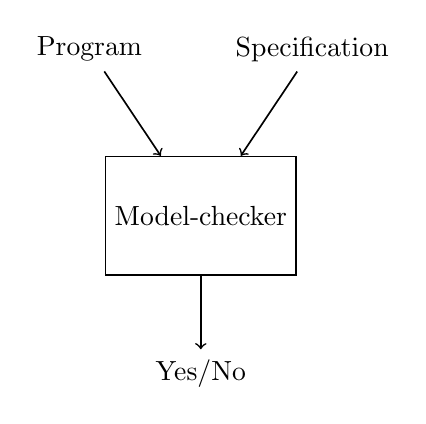
\begin{tikzpicture}[semithick,->,node distance=2cm]
  \node[draw, minimum height=15mm, minimum width=2cm] (MC) at (0,0) {Model-checker};
  \node (prog) [above=7mm, above left of=MC] {Program};
  \node (spec) [above=7mm, above right of=MC] {Specification};
  \node (result) [below of=MC] {Yes/No};
  \path (prog) edge (MC);
  \path (spec) edge (MC);
  \path (MC) edge (result);
  \end{tikzpicture}
\end{figure}
\end{frame}

%  There is bakery with only one clerk.
%  The clerk can serve only one customer at the time.
%  To avoid conflict between customers, a numbering machine gives a ticket to each customer.
%
%  \vspace{10pt}
%
%  What customers do:
%  {\small
%  \begin{enumerate}
%    \item Customer enters the bakery and get a ticket;
%    \item If he is alone or has the ticket with lowest number then he orders;
%    \item When he is done, he leaves the bakery and throws away the ticket.
%  \end{enumerate}
%  }
%
%  \vspace{10pt}
%
%  When the bakery is empty the numbering machine is reset.

%\section{Bakery Algorithm}
\begin{frame}
  \frametitle{Running example: Lamport's bakery algorithm}
  \vfill

  \begin{figure}[!h]
  \includegraphics[scale=0.4]{bakery}
  \end{figure}
  
  \vspace{1cm}
\end{frame}

\begin{frame}
  \frametitle{Running example: Lamport's bakery algorithm}
  \vfill
  
  \begin{figure}[!h]
  \includegraphics[scale=0.4]{order}
  \end{figure}
  
  \vspace{1cm}
\end{frame}

\begin{frame}
  \frametitle{Running example: Lamport's bakery algorithm}
  \vfill
  
  \begin{figure}[!h]
  \includegraphics[scale=0.4]{fight}
  \end{figure}
  
  \vspace{1cm}
\end{frame}

\begin{frame}
  \frametitle{Running example: Lamport's bakery algorithm}
  \vfill

  \begin{figure}[!h]
  \includegraphics[scale=0.4]{ticket}
  \end{figure}

  \vspace{1cm}
\end{frame}

\begin{frame}[fragile]
  \frametitle{Implementation of the algorithm for 2 customers.}
\begin{center}
{\footnotesize
initial state: pc1 = 0, x1 = 0, pc2 = 0, x2 = 0\\
pc values: (0 $\rightarrow$ outside), (1 $\rightarrow$ waiting), (2 $\rightarrow$ ordering)
}
\end{center}
\begin{minipage}{0.45\linewidth}
\begin{lstlisting}
while (true) {
  if(pc1 == 0){
    x1 = x2 + 1;
    pc1 = 1;
  }else if(pc1 == 1 &&
            (x2 == 0 ||
             x1 < x2 )){
    pc1 = 2;
  }else if(pc1 == 2){
    pc1 = 0;
    x1 = 0;
  }
  if(pc1==2 && pc2==2){
    ERROR;
  }
}
\end{lstlisting}
\end{minipage}
\hfill
\begin{minipage}{0.45\linewidth}
\begin{lstlisting}
while (true) {
  if(pc2 == 0){
    x2 = x1 + 1;
    pc2 = 1;
  }else if(pc2 == 1 &&
            (x1 == 0 ||
             x2 < x1 )){
    pc2 = 2;
  }else if(pc2 == 2){
    pc2 = 0;
    x2 = 0;
  }
  if(pc1==2 && pc2==2){
    ERROR;
  }
}
\end{lstlisting}
\end{minipage}
\end{frame}

\begin{frame}
  \frametitle{Why do we means by correct ?}
  safety: no two customers fight.
  
  \vspace{5mm}

  liveness: every customers eventually get served (starvation-free).

  \vspace{1cm}

  For this talk we will care only about \alert{safety} property.

\end{frame}

\begin{frame}
  \frametitle{The program as a dynamic system:}

  Initial state: $pc_1 = 0, x_1 = 0, pc_2 = 0, x_2 = 0$\\
 
  \hfill

  Transitions:
  \begin{tabular}{lcl}
    $pc_1=0$ & $\rightarrow$ & $pc_1'=1,~ x_1' = x_2 + 1$ \\
    $pc_1=1 \land (x_2=0 \lor x_1<x_2)$ & $\rightarrow$ & $pc_1'=2$ \\
    $pc_1=2$ & $\rightarrow$ & $pc_1' = 0,~ x_1' = 0$ \\
    & & \\
    $pc_2=0$ & $\rightarrow$ & $pc_2'=1,~ x_2' = x_1 + 1$ \\
    $pc_2=1 \land (x_1=0 \lor x_2<x_1)$ & $\rightarrow$ & $pc_2'=2$ \\
    $pc_2=2$ & $\rightarrow$ & $pc_2' = 0,~ x_2' = 0$ \\
    & & \\
    $pc_1=2 \land pc_2=2$ & $\rightarrow$ & ERROR
  \end{tabular}

\end{frame}

\begin{frame}
  \frametitle{Reachability graph:}

\parbox{1cm}{State:\\}
{\footnotesize
  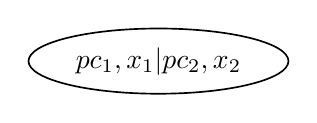
\begin{tikzpicture}[semithick,->,node distance=20mm, state/.style={draw,ellipse}]
  \node[state] (init) at (0,0) {$pc_1,x_1|pc_2,x_2$};
  \end{tikzpicture}
}

{\footnotesize
\begin{figure}
  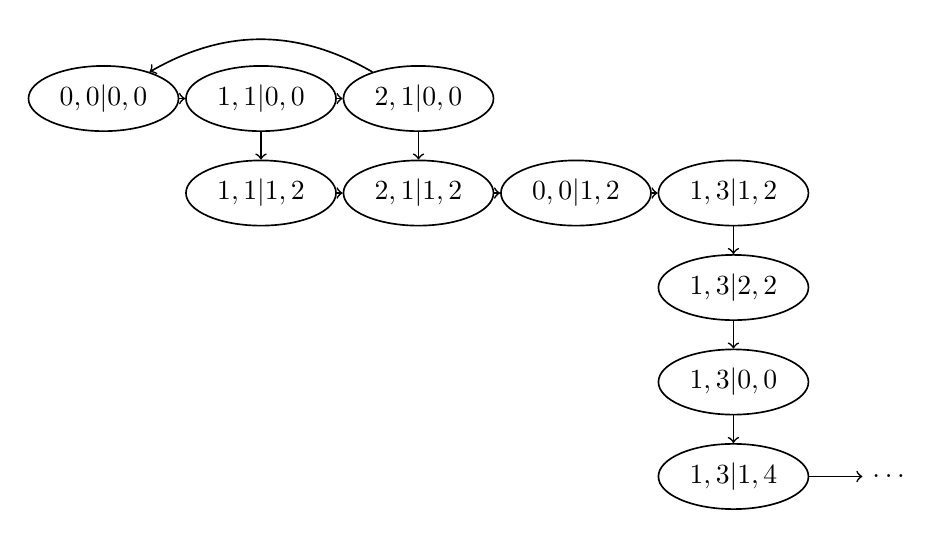
\begin{tikzpicture}[semithick,->,node distance=20mm, state/.style={draw,ellipse}]
  \node[state] (init) at (0,0) {$0,0|0,0$};
  
  \visible<2->{
    \node[state] (s1) [right of=init] {$1,1|0,0$};
    \path (init) edge (s1);
  }
  
  \visible<3->{
    \node[state] (s2) [right of=s1] {$2,1|0,0$};
    \path (s1) edge (s2);
  }

  \visible<4->{
    \path (s2) edge[bend right] (init);
  }

  \visible<5->{
    \node[state] (s3) [below=-8mm, below of=s1] {$1,1|1,2$};
    \path (s1) edge (s3);
  }
  \visible<6->{
    \node[state] (s4) [right of=s3] {$2,1|1,2$};
    \path (s3) edge (s4);
    \path (s2) edge (s4);
  }
  \visible<7->{
    \node[state] (s5) [right of=s4] {$0,0|1,2$};
    \path (s4) edge (s5);
  }
  \visible<8->{
    \node[state] (s6) [right of=s5] {$1,3|1,2$};
    \path (s5) edge (s6);
  }
  \visible<9->{
    \node[state] (s7) [below=-8mm, below of=s6] {$1,3|2,2$};
    \path (s6) edge (s7);
  }
  \visible<10->{
    \node[state] (s8) [below=-8mm, below of=s7] {$1,3|0,0$};
    \path (s7) edge (s8);
  }
  \visible<11->{
    \node[state] (s9) [below=-8mm, below of=s8] {$1,3|1,4$};
    \path (s8) edge (s9);
  }
  \visible<12->{
    \node (s10) [right of=s9] {$\dots$};
    \path (s9) edge (s10);
  }

  \end{tikzpicture}
\end{figure}
}
 
\visible<13->{
\begin{tikzpicture}[remember picture, overlay]
  \node[text width=6cm, fill=white, draw=red!80!black, very thick] (nw) at (current page.center) {
    The reachability graph is infinite.\\
    We cannot explore all of it.
  };
\end{tikzpicture}
}

\end{frame}

\begin{frame}
  \frametitle{The picture of abstraction}
  
  \begin{figure}
  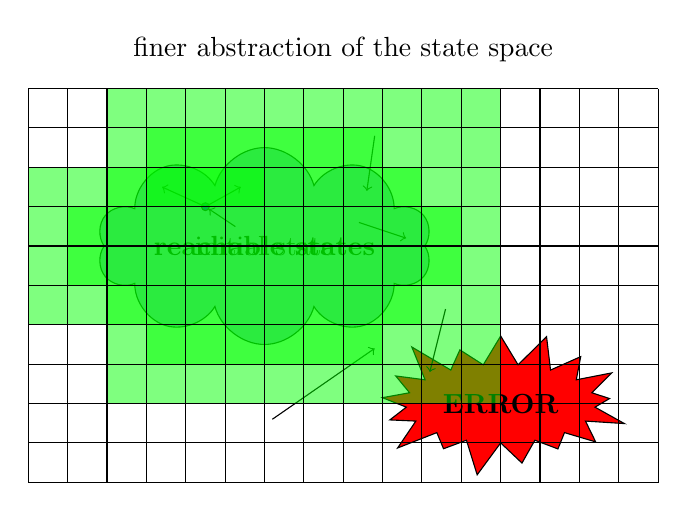
\begin{tikzpicture}
    \visible<2->{
      \node at (1,2.5) {state space};
      \draw[dashed] (-3,-3) rectangle (5,2);
    }
    \visible<5->{
      \node[cloud, cloud ignores aspect, draw, minimum width=3cm, minimum height=25mm, fill=blue!30] at (0,0) {\bf reachable states};
    }
    \visible<3->{
      \node[draw,circle,scale=0.3,fill=blue] (init) at (-0.75, 0.5) {};
      \node[starburst, draw, fill=red, minimum width=3cm, minimum height=2cm] at (3,-2) {\bf ERROR};
    }
    \visible<3>{
      \node (initText) at (0,0) {initial state};
      \path (initText) edge[->] (init);
    }
    %transitions
    \visible<4->{
      \draw[->] (-0.75,0.5) -- (-0.3,0.75);
      \draw[->] (-0.75,0.5) -- (-1.3,0.75);
      \draw[->] (1.2,0.3) -- (1.8,0.1);
      \draw[->] (1.4,1.4) -- (1.3,0.7);
      \draw[->] (0.1,-2.2) -- (1.4,-1.3);
      \draw[->] (2.3,-0.8) -- (2.1,-1.6);
    }
    %cover 1
    \visible<7-11>{ \path[fill=green, opacity=0.5] (-1,1) rectangle (0, 0); }
    \visible<8-11>{ \path[fill=green, opacity=0.5] (-2,1) rectangle (-1, 0); }
    \visible<9-11>{
      \path[fill=green, opacity=0.5] (-3,1) rectangle (-2, 0);
      \path[fill=green, opacity=0.5] (0,1) rectangle (3, 0);
    }
    \visible<10-11>{
      \path[fill=green, opacity=0.5] (-2,2) rectangle (3, 1);
      \path[fill=green, opacity=0.5] (-3,0) rectangle (3, -1);
    }
    \visible<11>{
      \path[fill=green, opacity=0.5] (-2,-1) rectangle (3, -2);
    }
    %grid 1
    \visible<6-11>{
      \node[fill=white] at (1,2.5) {finite abstraction of the state space};
      \draw (-3,-3) grid[xstep=1,ystep=1] (5,2);
    }
    %cover 2
    \visible<13,14>{ \path[fill=green, opacity=0.5] (-1,1) rectangle (-0.5, 0.5); }
    \visible<14>{
      \path[fill=green, opacity=0.5] (-1.5,1) rectangle (-1, 0.5);
      \path[fill=green, opacity=0.5] (-0.5,1) rectangle (0, 0.5);
    }
    \visible<15>{
      \path[fill=green, opacity=0.5] (-1.5  ,1.5) rectangle (1.5  , 1);
      \path[fill=green, opacity=0.5] (-2  ,1) rectangle (2  , 0.5);
      \path[fill=green, opacity=0.5] (-2.5,0.5) rectangle (2.5, -0.5);
      \path[fill=green, opacity=0.5] (-2  ,-0.5) rectangle (2  , -1);
      \path[fill=green, opacity=0.5] (-1.5  ,-1) rectangle (1.5  , -1.5);
    }
    %grid 2
    \visible<12->{
      \node[fill=white] at (1,2.5) {finer abstraction of the state space};
      \draw (-3,-3) grid[xstep=.5,ystep=.5] (5,2);
    }
  \end{tikzpicture}
  \end{figure}
\end{frame}

\begin{frame}
  \frametitle{Abstraction: preserving only some facts}
  problem: the range of $x_1$ and $x_2$ is infinite.

  \vspace{5pt}

  Maybe they are not important.
  
  \vfill

  Initial state: $pc_1 = 0, pc_2 = 0$
 
  \vspace{5pt}

  Transitions:

  \begin{tabular}{lcl}
    $pc_1=0$ & $\rightarrow$ & $pc_1'=1$ \\
    $pc_1=1$ & $\rightarrow$ & $pc_1'=2$ \\
    $pc_1=2$ & $\rightarrow$ & $pc_1'=0$ \\
    $pc_2=0$ & $\rightarrow$ & $pc_2'=1$ \\
    $pc_2=1$ & $\rightarrow$ & $pc_2'=2$ \\
    $pc_2=2$ & $\rightarrow$ & $pc_2'=0$ \\
    $pc_1=2 \land pc_2=2$ & $\rightarrow$ & ERROR
  \end{tabular}
  
  \vspace{10pt}

  The abstract system preserves traces, but adds new ones.

\end{frame}

\begin{frame}
  \frametitle{Abstract reachability graph}

{\footnotesize
\begin{figure}
  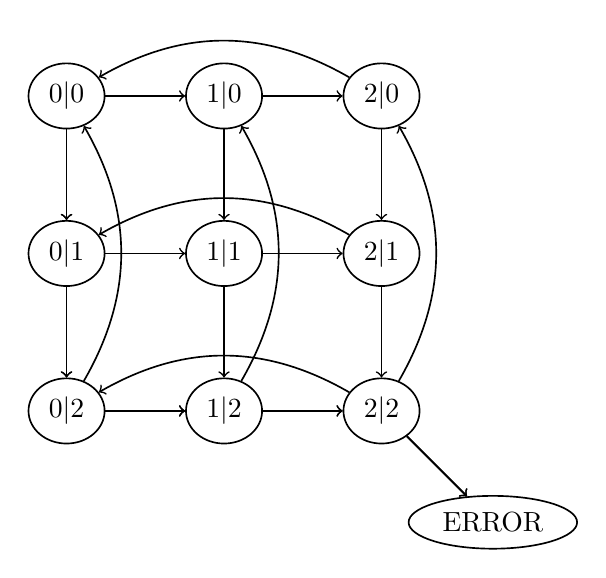
\begin{tikzpicture}[semithick,->,node distance=20mm, state/.style={draw,ellipse}]
  \node[state] (s00) at (0,0) {$0|0$};
  \node[state] (s10) [right of=s00] {$1|0$};
  \node[state] (s20) [right of=s10] {$2|0$};
  \node[state] (s01) [below of=s00] {$0|1$};
  \node[state] (s11) [right of=s01] {$1|1$};
  \node[state] (s21) [right of=s11] {$2|1$};
  \node[state] (s02) [below of=s01] {$0|2$};
  \node[state] (s12) [right of=s02] {$1|2$};
  \node[state] (s22) [right of=s12] {$2|2$};
  \node[state] (err) [below right of=s22] {ERROR};
  
  \visible<1>{
  \path (s00) edge (s01);
  \path (s01) edge (s02);
  \path (s02) edge[bend right] (s00);

  \path (s10) edge (s11);
  \path (s11) edge (s12);
  \path (s12) edge[bend right] (s10);

  \path (s20) edge (s21);
  \path (s21) edge (s22);
  \path (s22) edge[bend right] (s20);
  
  \path (s00) edge (s10);
  \path (s10) edge (s20);
  \path (s20) edge[bend right] (s00);

  \path (s01) edge (s11);
  \path (s11) edge (s21);
  \path (s21) edge[bend right] (s01);

  \path (s02) edge (s12);
  \path (s12) edge (s22);
  \path (s22) edge[bend right] (s02);

  \path (s22) edge (err);
  }

  \visible<2->{
  \path (s00) edge (s01);
  \path (s01) edge (s02);
  \path (s02) edge (s12);
  \path (s12) edge (s22);
  \path (s22) edge (err);
  }

  \end{tikzpicture}
\end{figure}
}
\end{frame}

\begin{frame}
  \frametitle{Analyzing the counterexample}
  
  \begin{minipage}[t]{0.45\linewidth}
    Abstract trace:

    \vspace{10pt}

  {\footnotesize
    $(pc_1=0|pc_2=0)$ \\
    \alert{$pc_2=0$ $\rightarrow$ $pc_2'=1$} \\
    $(pc_1=0|pc_2=1)$ \\
    \alert{$pc_2=1$ $\rightarrow$ $pc_2'=2$} \\
    $(pc_1=0|pc_2=2)$ \\
    \alert{$pc_1=0$ $\rightarrow$ $pc_1'=1$} \\
    $(pc_1=1|pc_2=2)$ \\
    \alert{$pc_1=1$ $\rightarrow$ $pc_1'=2$} \\
    $(pc_1=2|pc_2=2)$ \\
    \alert{$pc_1=2 \land pc_2=2$ $\rightarrow$ ERROR} \\
    ERROR
  }
  \end{minipage}
  \begin{minipage}[t]{0.5\linewidth}
    Concrete trace:

    \vspace{10pt}

  
  {\footnotesize
    \visible<2->{$(pc_1=0,x_1=0|pc_2=0,x_2=0)$} \\
    \visible<3->{\alert{$pc_2=0$ $\rightarrow$ $pc_2'=1,~ x_2' = x_1 + 1$} \\
    $(pc_1=0,x_1=0|pc_2=1,x_2=1)$} \\
    \visible<4->{\alert{$pc_2=1 \land (x_1=0 \lor x_2<x_1)$  $\rightarrow$  $pc_2'=2$} \\
    $(pc_1=0,x_1=0|pc_2=2,x_2=1)$} \\
    \visible<5->{\alert{$pc_1=0$  $\rightarrow$ $pc_1'=1,~ x_1' = x_2 + 1$} \\
    $(pc_1=1,x_1=2|pc_2=2,x_2=1)$} \\
    \visible<6->{\alert{$pc_1=1 \land (x_2=0 \lor x_1<x_2)$  $\rightarrow$  $pc_1'=2$}}
  }
  \end{minipage}

\visible<7->{
\begin{tikzpicture}[remember picture, overlay]
  \node[text width=6cm, fill=white, draw=red!80!black, very thick] (nw) at (current page.center) {
    The counterexample is spurious.\\
    The abstraction is too coarse.\\
    We need to add new facts.
  };
\end{tikzpicture}
}

\end{frame}

\begin{frame}
  \frametitle{Refinement: adding facts}
  We cannot track the exact ticket value.
  But we can remember who has the smallest number ($<,=,>$).
  
  \vfill

  Initial state: $pc_1 = 0, pc_2 = 0, x_1 = x_2$
 
  \vspace{10pt}

  Transitions:

  \begin{tabular}{lcl}
    $pc_1=0$ & $\rightarrow$ & $pc_1'=1,~ x_1' > x_2'$ \\
    $pc_1=1 \land (? \lor x_1 < x_2)$ & $\rightarrow$ & $pc_1'=2$ \\
    $pc_1=2$ & $\rightarrow$ & $pc_1' = 0,~ x_1' ~?~ x_2'$ \\
    $pc_2=0$ & $\rightarrow$ & $pc_2'=1,~  x_1' < x_2'$ \\
    $pc_2=1 \land (? \lor x_2 < x_1)$ & $\rightarrow$ & $pc_2'=2$ \\
    $pc_2=2$ & $\rightarrow$ & $pc_2' = 0,~ x_1' ~?~ x_2'$ \\
    $pc_1=2 \land pc_2=2$ & $\rightarrow$ & ERROR
  \end{tabular}

\end{frame}

\begin{frame}
  \frametitle{Abstract reachability graph}

  \alt<1,9->{
  \mbox{}~
  }{
  \alt<2>{
    $pc_1=0$ ~ $\rightarrow$ ~ $pc_1'=1,~ x_1' > x_2'$
  }{\alt<3>{
  $pc_1=1 \land (? \lor x_1 < x_2)$ ~ $\rightarrow$ ~ $pc_1'=2$
  }{\alt<4>{
  $pc_1=2$ ~ $\rightarrow$ ~ $pc_1' = 0,~ x_1' ~?~ x_2'$
  }{\alt<5>{
  $pc_2=0$ ~ $\rightarrow$ ~ $pc_2'=1,~  x_1' < x_2'$
  }{\alt<6>{
  $pc_2=1 \land (? \lor x_2 < x_1)$ ~ $\rightarrow$ ~ $pc_2'=2$ \\
  }{\alt<7>{
  $pc_1=2$ ~ $\rightarrow$ ~ $pc_1' = 0,~ x_1' ~?~ x_2'$ \\
  }{
  $pc_1=2 \land pc_2=2$ ~ $\rightarrow$ ~ ERROR
  }}}}}}}

{\tiny
\begin{figure}
  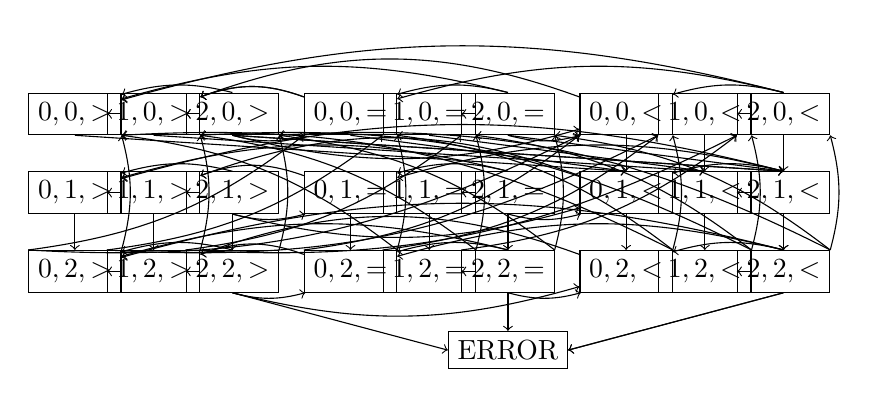
\begin{tikzpicture}[->,node distance=10mm, state/.style={draw}]
  \begin{scope}[xshift=-3.5cm]
    \node[state] (l00) at (0,0) {$0,0,>$};
    \node[state] (l10) [right of=l00] {$1,0,>$};
    \node[state] (l20) [right of=l10] {$2,0,>$};
    \node[state] (l01) [below of=l00] {$0,1,>$};
    \node[state] (l11) [right of=l01] {$1,1,>$};
    \node[state] (l21) [right of=l11] {$2,1,>$};
    \node[state] (l02) [below of=l01] {$0,2,>$};
    \node[state] (l12) [right of=l02] {$1,2,>$};
    \node[state] (l22) [right of=l12] {$2,2,>$};
  \end{scope}
  \begin{scope}
    \node[state] (e00) at (0,0) {$0,0,=$};
    \node[state] (e10) [right of=e00] {$1,0,=$};
    \node[state] (e20) [right of=e10] {$2,0,=$};
    \node[state] (e01) [below of=e00] {$0,1,=$};
    \node[state] (e11) [right of=e01] {$1,1,=$};
    \node[state] (e21) [right of=e11] {$2,1,=$};
    \node[state] (e02) [below of=e01] {$0,2,=$};
    \node[state] (e12) [right of=e02] {$1,2,=$};
    \node[state] (e22) [right of=e12] {$2,2,=$};
  \end{scope}
  \begin{scope}[xshift=3.5cm]
    \node[state] (g00) at (0,0) {$0,0,<$};
    \node[state] (g10) [right of=g00] {$1,0,<$};
    \node[state] (g20) [right of=g10] {$2,0,<$};
    \node[state] (g01) [below of=g00] {$0,1,<$};
    \node[state] (g11) [right of=g01] {$1,1,<$};
    \node[state] (g21) [right of=g11] {$2,1,<$};
    \node[state] (g02) [below of=g01] {$0,2,<$};
    \node[state] (g12) [right of=g02] {$1,2,<$};
    \node[state] (g22) [right of=g12] {$2,2,<$};
  \end{scope}
  \node[state] (err) [below of=e22] {ERROR};
  
  % $pc_1=0$ & $\rightarrow$ & $pc_1'=1,~ x_1' > x_2'$
  \visible<2,9>{
  \path (l00) edge                (l10);
  \path (l01) edge                (l11);
  \path (l02) edge                (l12);
  \path (e00) edge[bend right=20] (l10);
  \path (e01) edge[bend right=20] (l11);
  \path (e02) edge[bend right=20] (l12);
  \path (g00) edge[bend right=20] (l10);
  \path (g01) edge[bend right=20] (l11);
  \path (g02) edge[bend right=20] (l12);
  }

  % $pc_1=1 \land (? \lor x_1 < x_2)$ & $\rightarrow$ & $pc_1'=2$ \\
  \visible<3,9>{
  \path (l10) edge (l20);
  \path (l11) edge (l21);
  \path (l12) edge (l22);
  \path (e10) edge (e20);
  \path (e11) edge (e21);
  \path (e12) edge (e22);
  \path (g10) edge (g20);
  \path (g11) edge (g21);
  \path (g12) edge (g22);
  }
    
  % $pc_1=2$ & $\rightarrow$ & $pc_1' = 0,~ x_1' ~?~ x_2'$ \\
  \visible<4,9>{
  \path (l20.north) edge[bend right=15] (l00);
  \path (l20.south) edge[bend right=15] (e00);
  \path (l20.south) edge[bend right=15] (g00);
  \path (l21.north) edge[bend right=15] (l01);
  \path (l21.south) edge[bend right=15] (e01);
  \path (l21.south) edge[bend right=15] (g01);
  \path (l22.north) edge[bend right=15] (l02);
  \path (l22.south) edge[bend right=15] (e02);
  \path (l22.south) edge[bend right=15] (g02);
  \path (e20.north) edge[bend right=15] (l00);
  \path (e20.north) edge[bend right=15] (e00);
  \path (e20.south) edge[bend right=15] (g00);
  \path (e21.north) edge[bend right=15] (l01);
  \path (e21.north) edge[bend right=15] (e01);
  \path (e21.south) edge[bend right=15] (g01);
  \path (e22.north) edge[bend right=15] (l02);
  \path (e22.north) edge[bend right=15] (e02);
  \path (e22.south) edge[bend right=15] (g02);
  \path (g20.north) edge[bend right=15] (l00);
  \path (g20.north) edge[bend right=15] (e00);
  \path (g20.north) edge[bend right=15] (g00);
  \path (g21.north) edge[bend right=15] (l01);
  \path (g21.north) edge[bend right=15] (e01);
  \path (g21.north) edge[bend right=15] (g01);
  \path (g22.north) edge[bend right=15] (l02);
  \path (g22.north) edge[bend right=15] (e02);
  \path (g22.north) edge[bend right=15] (g02);
  }
  
  % $pc_2=0$ & $\rightarrow$ & $pc_2'=1,~  x_1' < x_2'$ \\
  \visible<5,9>{
  \path (l00.south) edge (g01.north);
  \path (l10.south) edge (g11.north);
  \path (l20.south) edge (g21.north);
  \path (e00.south) edge (g01.north);
  \path (e10.south) edge (g11.north);
  \path (e20.south) edge (g21.north);
  \path (g00) edge (g01);
  \path (g10) edge (g11);
  \path (g20) edge (g21);
  }

  % $pc_2=1 \land (? \lor x_2 < x_1)$ & $\rightarrow$ & $pc_2'=2$ \\
  \visible<6,9>{
  \path (l01) edge (l02);
  \path (l11) edge (l12);
  \path (l21) edge (l22);
  \path (e01) edge (e02);
  \path (e11) edge (e12);
  \path (e21) edge (e22);
  \path (g01) edge (g02);
  \path (g11) edge (g12);
  \path (g21) edge (g22);
  }
  
  % $pc_1=2$ & $\rightarrow$ & $pc_1' = 0,~ x_1' ~?~ x_2'$ \\
  \visible<7,9>{
  \path (l02.north east) edge[bend right=15] (l00.south east);
  \path (l02.north west) edge[bend right=15] (e00.south west);
  \path (l02.north west) edge[bend right=15] (g00.south west);
  \path (l12.north east) edge[bend right=15] (l10.south east);
  \path (l12.north west) edge[bend right=15] (e10.south west);
  \path (l12.north west) edge[bend right=15] (g10.south west);
  \path (l22.north east) edge[bend right=15] (l20.south east);
  \path (l22.north west) edge[bend right=15] (e20.south west);
  \path (l22.north west) edge[bend right=15] (g20.south west);
  \path (e02.north east) edge[bend right=15] (l00.south east);
  \path (e02.north east) edge[bend right=15] (e00.south east);
  \path (e02.north west) edge[bend right=15] (g00.south west);
  \path (e12.north east) edge[bend right=15] (l10.south east);
  \path (e12.north east) edge[bend right=15] (e10.south east);
  \path (e12.north west) edge[bend right=15] (g10.south west);
  \path (e22.north east) edge[bend right=15] (l20.south east);
  \path (e22.north east) edge[bend right=15] (e20.south east);
  \path (e22.north west) edge[bend right=15] (g20.south west);
  \path (g02.north east) edge[bend right=15] (l00.south east);
  \path (g02.north east) edge[bend right=15] (e00.south east);
  \path (g02.north east) edge[bend right=15] (g00.south east);
  \path (g12.north east) edge[bend right=15] (l10.south east);
  \path (g12.north east) edge[bend right=15] (e10.south east);
  \path (g12.north east) edge[bend right=15] (g10.south east);
  \path (g22.north east) edge[bend right=15] (l20.south east);
  \path (g22.north east) edge[bend right=15] (e20.south east);
  \path (g22.north east) edge[bend right=15] (g20.south east);
  }

  % $pc_1=2 \land pc_2=2$ & $\rightarrow$ & ERROR
  \visible<8,9>{
  \path (l22.south) edge (err.west);
  \path (e22.south) edge (err);
  \path (g22.south) edge (err.east);
  }
  
  \visible<10->{
  \path (e00) edge[bend right=20] (l10);
  \path (l10) edge (l20);
  \path (l20.south) edge (g21.north);
  \path (g21) edge (g22);
  \path (g22.south) edge (err.east);
  }
  
  \end{tikzpicture}
\end{figure}
}

\visible<11>{
\begin{tikzpicture}[remember picture, overlay]
  \node[text width=7cm, fill=white, draw=red!80!black, very thick] (nw) at (current page.center) {
    Too coarse again.\\
    We also need to track $x_1=0$ and $x_2=0$.
  };
\end{tikzpicture}
}

\end{frame}

\begin{frame}
  \frametitle{Safe abstract reachability graph}

\begin{minipage}{0.65\linewidth}
{\small
\begin{tabular}{l|ccccc}
id & pc1 & pc2 & $x_1=0$ & $x_2=0$ & $x_1 ? x_2$ \\
\hline
0  & 0  &  0  &  $\top$ & $\top$ & $x_1 = x_2$ \\
1  & 1  &  0  &  $\bot$ & $\top$ & $x_1 > x_2$ \\
2  & 0  &  1  &  $\top$ & $\bot$ & $x_1 < x_2$ \\
3  & 1  &  1  &  $\bot$ & $\bot$ & $x_1 < x_2$ \\
4  & 2  &  0  &  $\bot$ & $\top$ & $x_1 > x_2$ \\
5  & 0  &  2  &  $\top$ & $\bot$ & $x_1 < x_2$ \\
6  & 1  &  1  &  $\bot$ & $\bot$ & $x_1 > x_2$ \\
7  & 2  &  1  &  $\bot$ & $\bot$ & $x_1 < x_2$ \\
8  & 1  &  2  &  $\bot$ & $\bot$ & $x_1 > x_2$ \\
9  & 0  &  1  &  $\top$ & $\bot$ & $x_1 > x_2$ \\
10 & 1  &  0  &  $\bot$ & $\top$ & $x_1 < x_2$ \\
11 & 0  &  2  &  $\top$ & $\bot$ & $x_1 > x_2$ \\
12 & 2  &  0  &  $\bot$ & $\top$ & $x_1 < x_2$
\end{tabular}
}
\end{minipage}
\begin{minipage}{0.3\linewidth}
  \includegraphics[scale=0.3]{rg}
\end{minipage}

\end{frame}

\begin{frame}
  \frametitle{General idea:}

\begin{figure}
  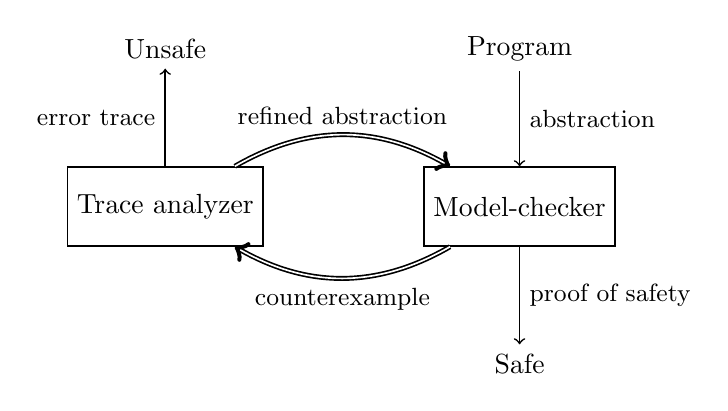
\begin{tikzpicture}[semithick,->,node distance=2cm]
  \node[draw, minimum height=10mm, minimum width=2cm] (MC) at (0,0) {Model-checker};
  \node (prog) [above of=MC] {Program};
  \node (safe) [below of=MC] {Safe};
  \node[draw, minimum height=10mm, minimum width=2cm] (trace) [left=25mm, left of=MC] {Trace analyzer};
  \node (error) [above of=trace] {Unsafe};

  \path (prog) edge node[right] {\small abstraction} (MC);
  \path (MC) edge node[right] {\small proof of safety} (safe);
  \path (MC) edge[double, bend left] node[below] {\small counterexample} (trace);
  \path (trace) edge[double, bend left] node[above] {\small refined abstraction} (MC);
  \path (trace) edge node[left] {\small error trace} (error);
  \end{tikzpicture}
\end{figure}

CEGAR: counterexample guided abstraction refinement

\end{frame}

\begin{frame}
\begin{center}
{\Huge
Questions ?
}

\vspace{2cm}

{\Large
Next part: The magic behind ``\emph{finding new facts}''
}

\vfill

{\scriptsize
(hard hat required)
}

\end{center}
\end{frame}

\begin{frame}[fragile]
  \frametitle{First iteration}

{\footnotesize
predicates: \\
initial state:
}
\vfill
\begin{minipage}{0.45\linewidth}
\begin{lstlisting}
while (true) {
  if(        ){
               ;
           ;
  }else if(         &&
            (        ||
                     )){
           ;
  }else if(        ){
           ;
          ;
  }
  if(       &&       ){
    ERROR;
  }
}
\end{lstlisting}
\end{minipage}
\hfill
\begin{minipage}{0.45\linewidth}
\begin{lstlisting}
while (true) {
  if(        ){
               ;
           ;
  }else if(         &&
            (        ||
                     )){
           ;
  }else if(        ){
           ;
          ;
  }
  if(       &&       ){
    ERROR;
  }
}
\end{lstlisting}
\end{minipage}

\visible<2->{
\begin{tikzpicture}[remember picture, overlay]
  \node (nw) at (current page.north west) {};
  \node (x) [below=12mm, below right of=nw] {};
  \draw[line width=2pt,double,->,color=red!90!black] (x) -- +(0,-4) .. controls +(0,-5) .. +(1,-5.3);
\end{tikzpicture}
}

\visible<3->{
\begin{tikzpicture}[remember picture, overlay]
  \node[text width=6cm, fill=white, draw, very thick] (nw) at (current page.center) {
    pc1 = 0, x1 = 0, pc2 = 0, x2 = 0;\\
    while (true) \{\\
    \mbox{}~~if(pc1==2 \&\& pc2==2)\{\\
    \mbox{}~~~~ERROR;\\
    \mbox{}~~\}\\
    \}
   };
\end{tikzpicture}
}

\end{frame}

\begin{frame}[fragile]
  \frametitle{First counterexample}
\begin{minipage}{0.45\linewidth}
\begin{lstlisting}[numbers=none]
pc1=0, x1=0, pc2=0, x2=0;
assume(pc1==2 && pc2==2);
ERROR;
\end{lstlisting}
\end{minipage}
\vfill
\begin{minipage}{0.8\linewidth}
SSA formula:
\begin{align*}
& \alert<2>{pc_1=0} \land x_1=0 \land pc_2=0 \land x_2=0 \\
& \alert<2>{pc_1=2} \land pc_2=2
\end{align*}
\visible<2>{Formula is unsat $\Rightarrow$ spurious counterexample}
\end{minipage}
\end{frame}

\begin{frame}
  \frametitle{Finding out why the cex is spurious.}

  Let $A$ and $B$ be two formulas such that
  $A \wedge B$ unsat.\\
  A [Craig] interpolant $I$ has the following properties:
  \begin{itemize}
  \item $I$ contains only $AB$-common symbols.
  \item $A$ implies $I$
  \item $I \wedge B$ unsat.
  \end{itemize}

\begin{align*}
& pc_1=0 \land x_1=0 \land pc_2=0 \land x_2=0 \\
& \hspace{8cm} \visible<2->{\alert{pc_1 = 0}}\\
& pc_1=2 \land pc_2=2
\end{align*}
\end{frame}

\begin{frame}[fragile]
  \frametitle{Second iteration}

{\footnotesize
predicates: pc1 = 0\\
initial state: pc1 = 0
}
\vfill
\begin{minipage}{0.45\linewidth}
\begin{lstlisting}
while (true) {
  if(pc1 == 0){
               ;
    pc1 = 1;
  }else if(pc1 == 1 &&
            (        ||
                     )){
    pc1 = 2;
  }else if(pc1 == 2){
    pc1 = 0;
          ;
  }
  if(pc1==2 &&       ){
    ERROR;
  }
}
\end{lstlisting}
\end{minipage}
\hfill
\begin{minipage}{0.45\linewidth}
\begin{lstlisting}
while (true) {
  if(        ){
               ;
           ;
  }else if(         &&
            (        ||
                     )){
           ;
  }else if(        ){
           ;
          ;
  }
  if(pc1==2 &&       ){
    ERROR;
  }
}
\end{lstlisting}
\end{minipage}

\visible<2>{
\begin{tikzpicture}[remember picture, overlay]
  \node (nw) at (current page.north west) {};
  \node (x) [below=15mm, below right of=nw] {};
  \draw[line width=2pt,double,->,color=red!90!black] (x) .. controls +(2,-0.75) .. +(0,-1.5) -- +(0,-4) .. controls +(0,-5) .. +(1,-5.3);
\end{tikzpicture}
}
\end{frame}

\begin{frame}[fragile]
  \frametitle{Second counterexample}
\begin{minipage}{0.45\linewidth}
\begin{lstlisting}[numbers=none]
pc1=0, x1=0, pc2=0, x2=0;
assume(pc1 == 0);
x1 = x2 + 1;
pc1 = 1;
assume(pc1==2 && pc2==2);
ERROR;
\end{lstlisting}
\end{minipage}
\vfill
\begin{minipage}{0.8\linewidth}
SSA formula:
\begin{align*}
& pc_1=0 \land x_1=0 \land pc_2=0 \land x_2=0 \\
& pc_1=0 \\
& x_1' = x_2 + 1 \\
& \alert<2>{pc_1' = 1} \\
& \alert<2>{pc_1'=2} \land pc_2=2
\end{align*}
\visible<2>{Formula is unsat $\Rightarrow$ spurious counterexample}
\end{minipage}
\end{frame}

\begin{frame}
  \frametitle{Finding out why the cex is spurious.}

\begin{align*}
& pc_1=0 \land x_1=0 \land pc_2=0 \land x_2=0 \\
& \hspace{8cm} \visible<2->{\top} \\
& pc_1=0 \\
& \hspace{8cm} \visible<3->{\top} \\
& x_1' = x_2 + 1 \\
& \hspace{8cm} \visible<4->{\top} \\
& pc_1' = 1 \\
& \hspace{8cm} \visible<5->{pc_1' = 1}\\
& pc_1'=2 \land pc_2=2
\end{align*}
\end{frame}

\begin{frame}[fragile]
  \frametitle{Third iteration}

{\footnotesize
predicates: pc1 = 0, pc1 = 1\\
initial state: pc1 = 0
}
\vfill
\begin{minipage}{0.45\linewidth}
\begin{lstlisting}
while (true) {
  if(pc1 == 0){
               ;
    pc1 = 1;
  }else if(pc1 == 1 &&
            (        ||
                     )){
    pc1 = 2;
  }else if(pc1 == 2){
    pc1 = 0;
          ;
  }
  if(pc1==2 &&       ){
    ERROR;
  }
}
\end{lstlisting}
\end{minipage}
\hfill
\begin{minipage}{0.45\linewidth}
\begin{lstlisting}
while (true) {
  if(        ){
               ;
           ;
  }else if(         &&
            (        ||
                     )){
           ;
  }else if(        ){
           ;
          ;
  }
  if(pc1==2 &&       ){
    ERROR;
  }
}
\end{lstlisting}
\end{minipage}

\begin{tikzpicture}[remember picture, overlay]
  \node (nw) at (current page.north west) {};
  \node (x) [below=15mm, below right of=nw] {};
  \node (y) [right of=x] {};
  \visible<2->{ \draw[line width=2pt,double,->,color=red!90!black] (x) .. controls +(1,-0.75) .. +(0,-1.5) -- +(0,-6); }
  \visible<3->{ \draw[line width=2pt,double,->,color=red!90!black] (y) -- +(0,-2) .. controls +(1,-2.5) .. +(0,-3) .. controls +(0,-5) .. +(1,-5.3); }
\end{tikzpicture}
\end{frame}

\begin{frame}[fragile]
  \frametitle{Third counterexample}
\begin{minipage}{0.65\linewidth}
\begin{lstlisting}[numbers=none]
pc1=0, x1=0, pc2=0, x2=0;
assume(pc1 == 0);
x1 = x2 + 1;
pc1 = 1;
assume(pc1==1 && (x1==0 || x2<x1));
pc1 = 2;
assume(pc1==2 && pc2==2);
ERROR;
\end{lstlisting}
\end{minipage}
\begin{minipage}{0.8\linewidth}
\begin{align*}
& pc_1=0 \land x_1=0 \land \alert<2>{pc_2=0} \land x_2=0 \\
& pc_1=0 \\
& x_1' = x_2 + 1 \\
& pc_1' = 1 \\
& pc_1'=1 \land (x_2=0 \lor x_1'<x_2) \\
& pc_1'' = 2 \\
& pc_1''=2 \land \alert<2>{pc_2=2}
\end{align*}
\visible<2>{Formula is unsat $\Rightarrow$ spurious counterexample}
\end{minipage}
\end{frame}

\begin{frame}[fragile]
  \frametitle{A few iterations later ...}

{\footnotesize
predicates: pc1 = 0, pc1 = 1, pc2 = 0, pc2 = 1\\
initial state: pc1 = 0, pc2 = 0
}
\vfill
\begin{minipage}{0.45\linewidth}
\begin{lstlisting}
while (true) {
  if(pc1 == 0){
               ;
    pc1 = 1;
  }else if(pc1 == 1 &&
            (        ||
                     )){
    pc1 = 2;
  }else if(pc1 == 2){
    pc1 = 0;
          ;
  }
  if(pc1==2 && pc2==2){
    ERROR;
  }
}
\end{lstlisting}
\end{minipage}
\hfill
\begin{minipage}{0.45\linewidth}
\begin{lstlisting}
while (true) {
  if(pc2 == 0){
               ;
    pc2 = 1;
  }else if(pc2 == 1 &&
            (        ||
                     )){
    pc2 = 2;
  }else if(pc2 == 2){
    pc2 = 0;
          ;
  }
  if(pc1==2 && pc2==2){
    ERROR;
  }
}
\end{lstlisting}
\end{minipage}

\begin{tikzpicture}[remember picture, overlay]
  \node (nw) at (current page.north west) {};
  \node (x) [below=15mm, below right of=nw] {};
  \node (y) [right of=x] {};
  \node (n) at (current page.north) {};
  \node (z) [below=12mm, below of=n] {};
  \node (a) [right of=z] {};
\visible<2->{ \draw[line width=2pt,double,->,color=red!90!black] (x) .. controls +(1,-0.75) .. +(0,-1.5) -- +(0,-6);}
\visible<3->{ \draw[line width=2pt,double,->,color=red!90!black] (y) -- +(0,-2) .. controls +(1,-2.5) .. +(0,-3) -- +(0,-6);}
\visible<4->{ \draw[line width=2pt,double,->,color=red!90!black] (z) .. controls +(1,-0.75) .. +(0,-1.5) -- +(0,-6);}
\visible<5->{ \draw[line width=2pt,double,->,color=red!90!black] (a) -- +(0,-2) .. controls +(1,-2.5) .. +(0,-3) .. controls +(0,-5) .. +(1,-5.3);}
\end{tikzpicture}
\end{frame}

\begin{frame}
  \frametitle{Finding out why the cex is spurious (first possibility)}

\begin{align*}
& pc_1=0 \land x_1=0 \land pc_2=0 \land x_2=0 \\
& \hspace{8cm} \visible<2->{x_2=0} \\
& pc_1=0 \land x_1' = x_2 + 1 \land pc_1' = 1 \\
& \hspace{8cm} \visible<3->{x_1' = 1 \land x_2 = 0} \\
& pc_1'=1 \land (x_2=0 \lor x_1'<x_2) \land pc_1'' = 2 \\
& \hspace{8cm} \visible<4->{x_1' = 1}\\
& pc_2=0 \land x_2' = x_1' + 1 \land pc_2' = 1 \\
& \hspace{8cm} \visible<5->{x_1' = 1 \land x_2' = 2} \\
& pc_2'=1 \land (x_1'=0 \lor x_2'<x_1') \land pc_2'' = 2 \\
& \hspace{8cm} \visible<6->{\bot}\\
& pc_1''=2 \land pc_2''=2
\end{align*}
\end{frame}


\begin{frame}[fragile]
  \frametitle{Does it work ?}

{\footnotesize
predicates: pc1 = 0, pc1 = 1, pc2 = 0, pc2 = 1, x1=1, x2=0, x2=2\\
initial state: pc1 = 0, x1 = 0, pc2 = 0, x2 = 0
}
\vfill
\begin{minipage}{0.45\linewidth}
\begin{lstlisting}
while (true) {
  if(pc1 == 0){
    x1 = x2 + 1;
    pc1 = 1;
  }else if(pc1 == 1 &&
            (x2 == 0 ||
             x1 < x2 )){
    pc1 = 2;
  }else if(pc1 == 2){
    pc1 = 0;
    x1 = 0;
  }
  if(pc1==2 && pc2==2){
    ERROR;
  }
}
\end{lstlisting}
\end{minipage}
\hfill
\begin{minipage}{0.45\linewidth}
\begin{lstlisting}
while (true) {
  if(pc2 == 0){
    x2 = x1 + 1;
    pc2 = 1;
  }else if(pc2 == 1 &&
            (x1 == 0 ||
             x2 < x1 )){
    pc2 = 2;
  }else if(pc2 == 2){
    pc2 = 0;
    x2 = 0;
  }
  if(pc1==2 && pc2==2){
    ERROR;
  }
}
\end{lstlisting}
\end{minipage}

\begin{tikzpicture}[remember picture, overlay]
  \node (nw) at (current page.north west) {};
  \node (x1) [below=15mm, below right of=nw] {};
  \node (x2) [right of=x1] {};
  \node (x3) [right of=x2] {};
  \node (x4) [right of=x3] {};
  \node (x5) [right of=x4] {};
  \node (n) at (current page.north) {};
  \node (y1) [below=12mm, below of=n] {};
  \node (y2) [right of=y1] {};
  \node (y3) [right of=y2] {};
  \node (y4) [right of=y3] {};
  \node (y5) [right of=y4] {};
\visible<2->{ \draw[line width=2pt,double,->,color=red!90!black] (x1) .. controls +(1,-0.75) .. +(0,-1.5) -- +(0,-6); }
\visible<3->{ \draw[line width=2pt,double,->,color=red!90!black] (x2) -- +(0,-2) .. controls +(1,-2.5) .. +(0,-3) -- +(0,-6);}
\visible<4->{ \draw[line width=2pt,double,->,color=red!90!black] (y1) .. controls +(1,-0.75) .. +(0,-1.5) -- +(0,-6);}
\visible<5->{ \draw[line width=2pt,double,->,color=red!90!black] (x3) -- +(0,-3.5) .. controls +(1,-4) .. +(0,-4.5) -- +(0,-6);}
\visible<6->{ \draw[line width=2pt,double,->,color=red!90!black] (x4) .. controls +(1,-0.75) .. +(0,-1.5) -- +(0,-6); }
\visible<7->{ \draw[line width=2pt,double,->,color=red!90!black] (y2) -- +(0,-2) .. controls +(1,-2.5) .. +(0,-3) -- +(0,-6);}
\visible<8->{ \draw[line width=2pt,double,->,color=red!90!black] (y3) -- +(0,-3.5) .. controls +(1,-4) .. +(0,-4.5) -- +(0,-6);}
\visible<9->{ \draw[line width=2pt,double,->,color=red!90!black] (y4) .. controls +(1,-0.75) .. +(0,-1.5) -- +(0,-6); }
\visible<10->{ \draw[line width=2pt,double,->,color=red!90!black] (x5) -- +(0,-2) .. controls +(1,-2.5) .. +(0,-3) -- +(0,-6);}
\visible<11->{ \draw[line width=2pt,double,->,color=red!90!black] (y5) -- +(0,-2) .. controls +(1,-2.5) .. +(0,-3) .. controls +(0,-5) .. +(1,-5.3);}
\end{tikzpicture}
\end{frame}

\begin{frame}
  \frametitle{Finding out why the cex is spurious (second possibility)}

\begin{align*}
& pc_1=0 \land x_1=0 \land pc_2=0 \land x_2=0 \\
& \hspace{8cm} \visible<2->{x_2=0} \\
& pc_1=0 \land x_1' = x_2 + 1 \land pc_1' = 1 \\
& \hspace{8cm} \visible<3->{x_1' > x_2 \land x_2 = 0} \\
& pc_1'=1 \land (x_2=0 \lor x_1'<x_2) \land pc_1'' = 2 \\
& \hspace{8cm} \visible<4->{x_1' > 0}\\
& pc_2=0 \land x_2' = x_1' + 1 \land pc_2' = 1 \\
& \hspace{8cm} \visible<5->{x_1' > 0 \land x_2' > x_1'} \\
& pc_2'=1 \land (x_1'=0 \lor x_2'<x_1') \land pc_2'' = 2 \\
& \hspace{8cm} \visible<6->{\bot}\\
& pc_1''=2 \land pc_2''=2
\end{align*}
\end{frame}

\begin{frame}[fragile]
  \frametitle{Final version}

{\footnotesize
predicates: pc1=0, pc1=1, pc2=0, pc2=1, x1=0, x2=0, x1$<$x2, x1$>$x2\\
initial state: pc1 = 0, x1 = 0, pc2 = 0, x2 = 0
}
\vfill
\begin{minipage}{0.45\linewidth}
\begin{lstlisting}
while (true) {
  if(pc1 == 0){
    x1 = x2 + 1;
    pc1 = 1;
  }else if(pc1 == 1 &&
            (x2 == 0 ||
             x1 < x2 )){
    pc1 = 2;
  }else if(pc1 == 2){
    pc1 = 0;
    x1 = 0;
  }
  if(pc1==2 && pc2==2){
    ERROR;
  }
}
\end{lstlisting}
\end{minipage}
\hfill
\begin{minipage}{0.45\linewidth}
\begin{lstlisting}
while (true) {
  if(pc2 == 0){
    x2 = x1 + 1;
    pc2 = 1;
  }else if(pc2 == 1 &&
            (x1 == 0 ||
             x2 < x1 )){
    pc2 = 2;
  }else if(pc2 == 2){
    pc2 = 0;
    x2 = 0;
  }
  if(pc1==2 && pc2==2){
    ERROR;
  }
}
\end{lstlisting}
\end{minipage}
\end{frame}


%\section*{Conclusion}
\begin{frame}

\begin{center}
\Huge
Questions ?
\end{center}
\end{frame}


\end{document}
